% !TEX encoding = UTF-8
% !TEX TS-program = pdflatex
% !TEX root = ../apprendimento_automatico.tex
% !TEX spellcheck = it-IT
\section{Lezione 10 - Reti neurali 2}\label{lezione-10---reti-neurali-2}

Perceptron va bene ma non riesce ad apprendere la XOR perché non è
linearmente separabile.

\subsection{Reti di Perceptron}\label{reti-di-perceptron}

L'idea è quindi quella di combinare più Perceptron tra loro, in modo che
riescano ad apprendere una qualsiasi funzione boolena.

Il problema ora diventa come effettuare l'apprendimento con una rete di
Perceptron, dal momento che non è più triviale come assegnare dei pesi
alle unità nascoste. Una possibile soluzione è quella di rendere il
singolo neurone derivabile e sfruttare la tecnica di Discesa del
Gradiente per apprendere i pesi ``giusti''.

\subsubsection{Discesa di gradiente}\label{discesa-di-gradiente}

\textbf{Richiami di analisi}: il segno della derivata di una funzione
determina se la funzione è crescente o decrescente. Inoltre se la
derviata vale 0, la funzione in quel punto ha un minimo o un massimo
locale.

Si può quindi seguire il segno della derivata prima di una funzione per
raggiungere un massimo o minimo locale.

Per vedere come funziona la discesa di gradiente conviene considerare un neurone senza Threshold o sigmoide, ovvero un neurone che esegue solamente il prodotto scalare tra il vettore dei pesi e degli ingressi.

La funzione \textit{out} diventa quindi:

$$
out(\vec{x}) = \sum\limits_{i=0}^n w_i \cdot x_i = \vec{w} \cdot \vec{x}
$$

La discesa di gradiente viene utilizzata per minimizzare l'errore empirico commesso dal neurone nel valutare un esempio del training set utilizzando un determinato vettore di pesi.

$$
E(\vec{w}) = \frac{1}{2} \sum_{(\vec{x},t) \in Tr} (t - out(\vec{x}))^2
$$

Le slide del corso utilizzano $\frac{1}{2 \cdot N_{Tr}}$ al posto di $\frac{1}{2}$ dove $N_{Tr}$ è la cardinalità dell'insieme di apprendimento.
La mancanza di questo fattore non influisce sulla correttezza delle formule dal momento che si sta affrontando un problema di minizzazione.

L'algoritmo parte quindi da un $\vec{w}$ generato casualmente e cerca di modificarlo nella direzione contraria al gradiente della funzione errore, in modo da minimizzarla.

$$
\nabla E[\vec{w}] \equiv \left[ \frac{\partial E}{\partial w_0}, \frac{\partial E}{\partial w_1}, \ldots, \frac{\partial E}{\partial w_n}  \right] 
$$

Una volta calcolato il gradiente è possibile calcolare il valore per aggiornare il vettore dei pesi:

$$
\Delta\vec{w} = -\eta \nabla E[\vec{w}] \text{ ovvero } \Delta w_i = -\eta \frac{\partial E}{\partial w_i} \qquad \forall i
$$

Il valore $\eta$ è lo step con il quale l'algoritmo si sposta verso il minimo e prende il nome di
\textbf{learn rate}.

Per calcolare lo spostamento rispetto ad ogni $w_i$ per minimizzare
la funzione obiettivo è necessario calcolare la derivata della funzione errore. 

\begin{align*}
\frac{\partial E}{\partial w_i} &= \frac{\partial}{\partial w_i} \frac{1}{2} \sum_{(\vec{x},t) \in Tr} (t - out(\vec{x}))^2 \\
	&= \text{\textit{*magic*}} \\
	&= - \sum_{(\vec{x},t) \in Tr} (t - out(\vec{x}))(x_i) \\
\end{align*}

\paragraph{Algoritmo di apprendimento}\label{algoritmo-di-apprendimento}

$\Delta w_i$ rappresenta lo spostamento dal $w_i$ iniziale.

\begin{enumerate}
\item Assegna a $w_i$ dei valori casuali vicini allo 0
\item Finché non si verifica la condizione di terminazione
	\begin{enumerate}
	\item $\Delta w_i \leftarrow 0$
	\item Per ogni esempio del training set $(\vec{x},t)$:
		\begin{enumerate}
		\item Calcola $out(\vec{x})$
		\item Aggiorna il vettore $\Delta w$:  $\Delta w_i \leftarrow \Delta w_i + \eta (t - out(\vec{x}))x_i$
		\end{enumerate}
	\end{enumerate}
	\item Aggiorna il vettore dei pesi \textit{w}: $w_i \leftarrow w_i + \Delta w_i$
\end{enumerate}

In pratica prima viene esaminato tutti il training set per calcolare i
vari $\Delta w_i$, una volta finito di esaminare il training set si
aggiornano i $w_i$ e si ripete fino a che non si verifica una
condizione di stop.

Possono essere utilizzate varie condizioni di stop:

\begin{itemize}
\item
  $E[\vec{w}]$ minore di una soglia prefissata
\item
  $\Delta w_i = 0 \: \forall i$
\item
  Il numero di iterazioni ha superato una soglia prefissata.
\end{itemize}

\subsubsection{Discesa di gradiente con sigmoide}\label{discesa-di-gradiente-con-sigmoide}

Per utilizzare l'algoritmo di discesa di gradiente con un neurone sigmoidale è necessario effettuare qualche piccola modifica dovuta al fatto che cambia la funzione che viene calcolata dal neurone.

$$
out(\vec{x}) = \sigma (\sum\limits_{i = 0}^n w_i \cdot x_i ) = \sigma(\vec{w} \cdot \vec{x})
$$

dove:

\begin{align*}
\sigma(net) &= \frac{1}{1 + e^{-net}} \\
\frac{\partial \sigma}{\partial net} &= \sigma(net)(1-\sigma(net))
\end{align*}

La differenza riguarda il calcolo di $\frac{\partial E}{\partial w_i}$ che diventa:

\begin{align*}
\frac{\partial E}{\partial w_i} &= \frac{\partial}{\partial w_i} \frac{1}{2} \sum_{(\vec{x},t) \in Tr} (t - out(\vec{x}))^2 \\
	&= \text{\textit{*magic*}} \\
	&= - \sum_{(\vec{x},t) \in Tr} (t - out(\vec{x})) \sigma(\vec{w} \cdot \vec{x})(1-\sigma(\vec{w} \cdot \vec{x}))\cdot x_i \\
	&= - \sum_{(\vec{x},t) \in Tr} (t - out(\vec{x})) out(\vec{x})  (1-out(\vec{x})) x_i \\
\end{align*}

e di conseguenza la formula di aggiornamento per $\Delta w_i$ risulta essere:

$$
\Delta w_i \leftarrow \Delta w_i + \eta (t - out(\vec{x})) out(\vec{x})  (1-out(\vec{x})) x_i
$$
\subsection{Rete di Perceptron}\label{rete-di-perceptron}

\begin{figure}[htbp]
\centering
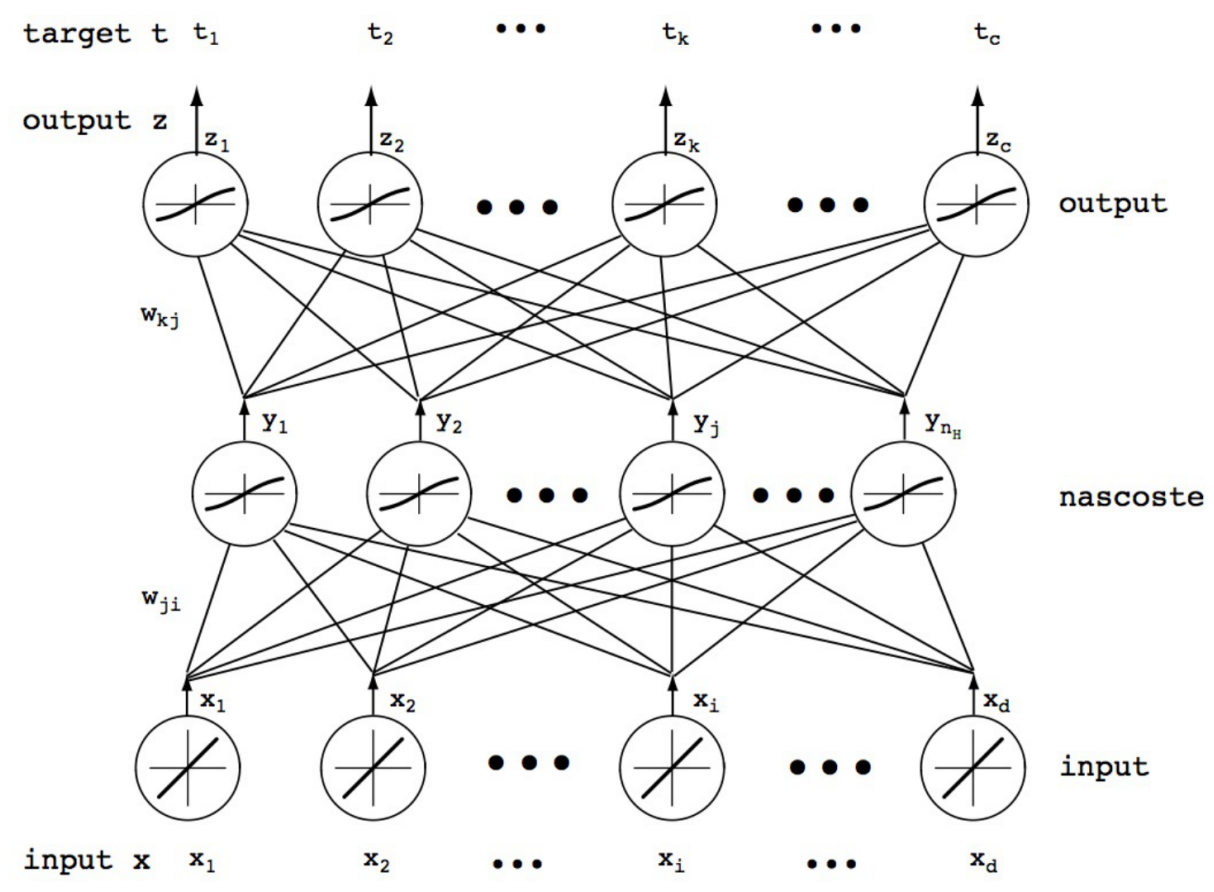
\includegraphics[width=\textwidth]{./notes/immagini/l10-rete.png}
\caption{Rete neurale}
\end{figure}

Una generica rete neurale è composta da:

\begin{itemize}
\item \textit{d} unità di ingresso che corrispondo a $\vec{x} \equiv (x_1, \cdots, x_d)$
\item $N_H$ unità nascoste, ognuna con output $\vec{y} \equiv (y_1, \cdots, y_{N_H})$
\item \textit{c} unità di output che corrispondo a $\vec{z} \equiv (z_1, \cdots, z_c)$ e che rappresentano dati del tipo $\vec{t} \equiv (t_1, \cdots, t_c)$ .
\item $w_{j,i}$ peso dall'unità di ingresso \textit{i} all'unità nascosta \textit{j}.
\item $w_{k,j}$ peso dall'unità nascosta \textit{j} all'unità d'uscita \textit{k}.
\end{itemize}

La funzione che rappresenta l'errore commesso dalla rete è:

$$
E[\vec{w}] = \frac{1}{2c} \sum\limits_{(\vec{x}. \vec{t}) \in Tr} \sum\limits_{k=1}^c (t_k - z_k(\vec{x}))^2
$$

Ovvero risulta essere la sommatoria dei quadrati degli errori compiuti dalle singole unità di output.

\subsubsection{Calcolo dei pesi per le unità di output}\label{calcolo-dei-pesi-per-le-unituxe0-di-output}

Per calcolare l'aggiornamento dei pesi delle unità di output, viene tenuto in considerazione solamente il livello nascosto che alimenta.

\begin{figure}[htbp]
\centering
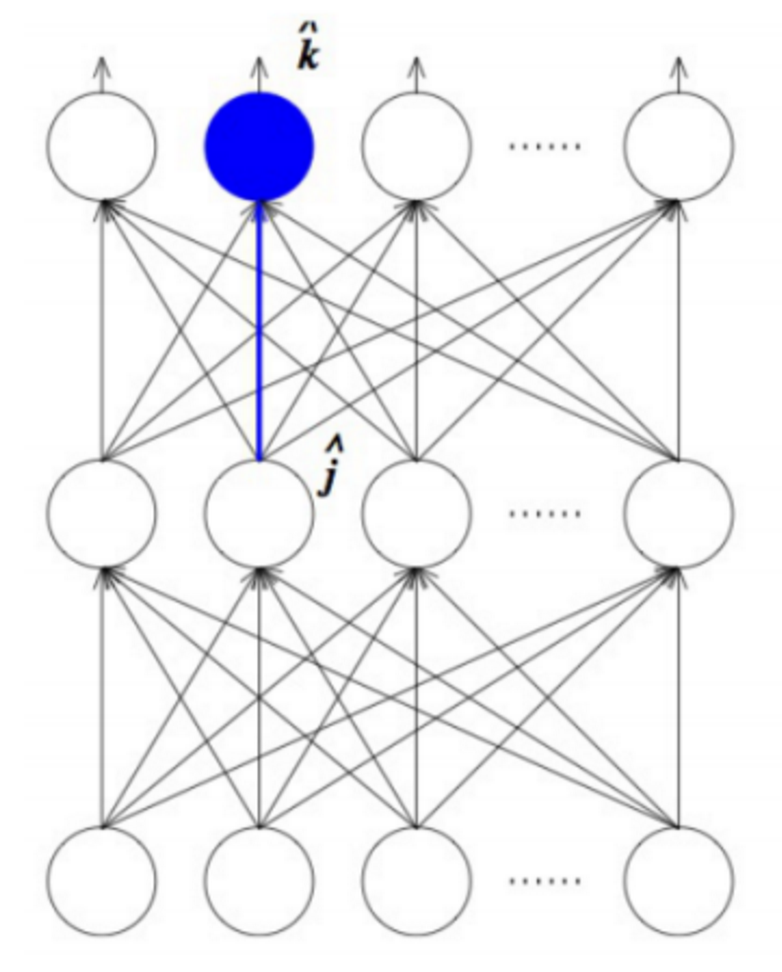
\includegraphics[width=0.4\textwidth]{./notes/immagini/l10-wkj.png}
\caption{Neuroni coinvolti per il calcolo di $\frac{\partial E}{\partial w_{\hat{k},\hat{j}}}$}
\end{figure}

La formula per l'aggiornamento del componente $\hat{j}$ del vettore dei pesi per l'unità $\hat{k}$, risulta essere:

\begin{align*}
\frac{\partial E}{\partial w_{\hat{k},\hat{j}}} &= \frac{\partial}{\partial w_{\hat{k},\hat{j}}} \frac{1}{2c} \sum_{(\vec{x},t) \in Tr} \sum\limits_{k=1}^c (t_k - z_k(\vec{x}))^2 \\
 &= \text{\textit{*magic*}} \\
 &= - \frac{1}{c} \sum_{(\vec{x},t) \in Tr} (t_{\hat{k}} - z_{\hat{k}}(\vec{x}))\sigma ' (\vec{w}_{\hat{k}}  \cdot \vec{y}) y_{\hat{j}} 
\end{align*}

\subsubsection{Calcolo dei pesi per le unità nascoste}\label{calcolo-dei-pesi-per-le-unituxe0-nascoste}

\begin{figure}[htbp]
\centering
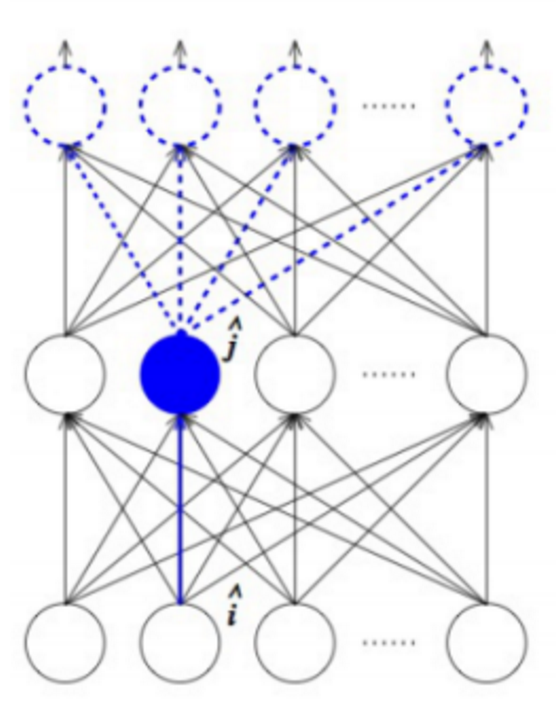
\includegraphics[width=0.4\textwidth]{./notes/immagini/l10-wji.png}
\caption{Neuroni coinvolti per il calcolo di $\frac{\partial E}{\partial w_{\hat{j},\hat{k}}}$}
\end{figure}

La formula per l'aggiornamento del componente $\hat{i}$ del vettore dei pesi per l'unità $\hat{j}$, risulta essere:

\begin{align*}
\frac{\partial E}{\partial w_{\hat{j},\hat{i}}} &= \frac{\partial}{\partial w_{\hat{j},\hat{i}}} \frac{1}{2c} \sum_{(\vec{x},t) \in Tr} \sum\limits_{k=1}^c (t_k - z_k(\vec{x}))^2 \\
 &= \text{\textit{*magic*}} \\
 &= - \frac{1}{c} \sum_{(\vec{x},t) \in Tr} \sum\limits_{k=1}^c (t_{k} - z_{k}(\vec{x}))  \sigma ' (\vec{w}_{k}  \cdot \vec{y}) \sigma ' (\vec{w}_{\hat{j}}  \cdot \vec{x}) x_{\hat{i}}
\end{align*}

Da notare che il risultato finale viene influenzato anche dai pesi che collegano il livello nascosto con il resto della rete, ovvero $\sigma ' (\vec{w}_{k}  \cdot \vec{y}) $.

Rimane inoltre valido che $\sigma ' (\vec{w}_{k}  \cdot \vec{y}) = \sigma  (\vec{w}_{k}  \cdot \vec{y}) (1 - \sigma ' (\vec{w}_{k}  \cdot \vec{y}))$

\subsubsection{Algoritmo di apprendimento}\label{algoritmo-di-apprendimento-1}

L'algoritmo di apprendimento che prende il nome di \textbf{Back Propagation stocastico} lavora in due fasi: nella prima fase, detta
\textbf{feed forward}, viene fornito in input alla rete un esempio del
training set, in modo che questa possa provare a calcolare la funzione
target per l'esempio. 

Una volta calcolata si passa alla fase di
\textbf{backward progragation}, nella quale si aggiornano i coefficienti
delle unità di output e delle unità nascoste in base alla correttezza o
meno della predizione. In questo caso l'apprendimento avviene a ritroso,
prima vengono aggiornati i coefficienti delle unità di output e poi
quelli dei livelli nascosti.

\begin{enumerate}
\item Inizializzazione di tutti i pesi con dei valori casuali ma vicini allo 0.
\item Per ogni esempio del training set $(\vec{x},\vec{t})$:
	\begin{enumerate}
	\item Usa la rete neurale per calcolare $\vec{o} = out(\vec{x})$
	\item Per ogni unità di output \textit{k}: 
	$$\delta_k \leftarrow \underbrace{(t_k - o_k)}_{\text{differenza tra l'output atteso e quello ottenuto}} \cdot \overbrace{o_k \cdot (1 - o_k)}^{\text{derivata prima della funzione } out(\vec{x})}$$
	
	\item Per ogni unità nascosta \textit{j}: 
	$$\delta_j \leftarrow \overbrace{o_j \cdot (1 - o_j)}^{\text{derivata prima della funzione } out(\vec{x})} \underbrace{\sum_{k \in outputs} w_{k,j}\delta_k}_{\text{peso delle connessioni in uscita aggiornato}}$$
	
	\item Aggiorna tutti i pesi $w_{s,q}$ della rete con:
	$$ w_{s,q} \leftarrow w_{s,q} + \eta \Delta w_{s,q}$$
	dove
	$$
	\Delta w_{s,q} = 
		\begin{cases}
        	\delta_s x_q,& \text{se } s \in nascoste\\
    		\delta_s y_q,& \text{se } s \in output\\
		\end{cases}
	$$
	\end{enumerate}
\end{enumerate}

Il passo \textit{(b)} dell'algoritmo rappresenta il calcolo della differenza tra
l'output atteso e quello ottenuto, questo viene poi utilizzato per
aggiornare a ritroso i valori dei nodi interni (passo \textit{(c)}).

L'algoritmo prende il nome di \textbf{back propagation stocastico}
perché il valore dei $\Delta w_{s,q}$ viene aggiornato subito dopo aver
valutato un esempio \emph{x} e non dopo aver valutato tutti
gli esempi del training set.

Le possibili condizioni di terminazione sono le stesse che si hanno
quando c'è un solo neurone.
